\chapter{Analysis of PbS QD simulation data}

In this chapter we will take a look at the simulation data. The parameters used for the simulation can be found in appendix~\ref{A}. We will make an analysis of the energy levels and wave functions of PbS QDs and draw some conclusions.\\

\begin{REMARK} 
There are a few practical aspects to note concerning the simulation of PbS QDs with \omen: Since \omen will consider in its calculation 18 orbitals for the atoms, one must keep in mind that the simulation uses significantly more computing resources than a simulation of, for instance, a CdSe-CdS QD. Especially the memory usage during the calculation can easily exceed 10GB for larger QDs. The size of the generated simulation data for one QD can also amount to more than a few 100MB. It has to be kept in mind, that the number of atoms scales with the third potence of the radius. Another problem is the high degeneracy of energy levels. This makes it necessarry to simulate a higher number of modes, thus increasing the usage of resources further.
\end{REMARK}

\section{Energy leves}
%ENERGY LEVELS

%FIGURES
\begin{figure}
	\centering
	\begin{subfigure}{60px}
		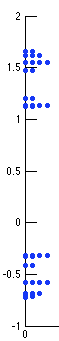
\includegraphics[height=150px]{Fig/Plots/r1b.png}
		\caption{}
	\end{subfigure}    
	\begin{subfigure}{60px}
		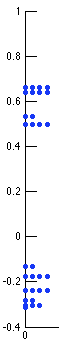
\includegraphics[height=150px]{Fig/Plots/r3b.png}
		\caption{}
	\end{subfigure}
	\begin{subfigure}{60px}
		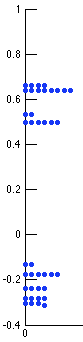
\includegraphics[height=150px]{Fig/Plots/r3a.png}
		\caption{}
	\end{subfigure}
	\begin{subfigure}{60px}
		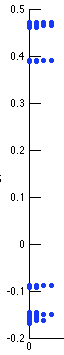
\includegraphics[height=150px]{Fig/Plots/r5b.png}
		\caption{}
	\end{subfigure}    
	\begin{subfigure}{60px}
		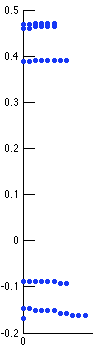
\includegraphics[height=150px]{Fig/Plots/r5a.png}
		\caption{}
	\end{subfigure}
	\caption{Energy levels for different sized QDs: 2nm (a), 6nm (b) and (c), 10nm (d) and (e). Vertical axis in eV. Multiple dots on the horizontal axis signify degeneracy. In plots (c) and (e) energies within 0.03eV are plottet as degenerate, for better visibility.}
	\label{fig:e-levels}	
\end{figure}

\begin{figure}
	\centering
	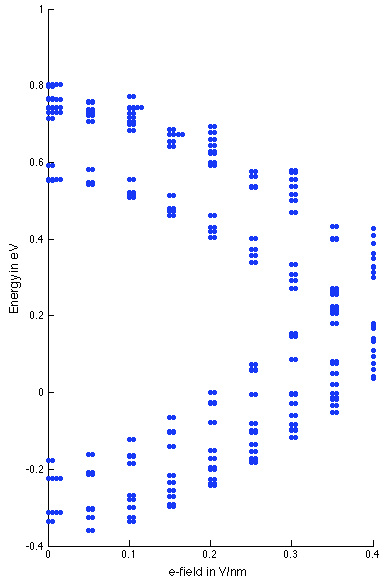
\includegraphics[width=200px]{Fig/Plots/r25v.png}
	\caption{Energy states (including degeneracy) for different electric fields.}
	\label{fig:EvsVolt}
\end{figure}


% TEXT
\begin{REMARK}
In the following discussion, the terms conduction band, band edge and so on are used. Although there are no energy bands present in a QD, but rather discrete energy levels, these terms nevertheless make sense, since the states above the band gap are similar to conduction band states, and those below to valence band states, respectively. Indeed, if the QD gets bigger, we finally reach the limit where we can treat it as a bulk material. The term \textit{conduction band} thus refers in this context to the discrete energy states above the band gap.
\end{REMARK}
	
Taking a look at the eigenenergies close to the bandedge, one can see that there are 8 closely spaced modes, for conduction and valence band respectively. Generally, closest to the band edge there is a twofold degenerate energy level, followed by a fourfold degenerate level and then again a twofold degenerate level. (For a few simulations the order is different, for example the fourfold degenerate energy level is closest to the band edge.)
	
As the size of the QDs increases, the energy levels get closer to each other, resulting in higher degeneracy. This is shown in figure~\ref{fig:e-levels} (a),(b),(d), where the energy levels (including degeneracy) are shown for 2, 6 and 10nm QDs. Since some levels are very closely spaced, they are not clearly distinguishable form each other. For this reason, the tolerance, within which an energy level is shown as degenerate, was increased in figure~\ref{fig:e-levels} (c),(e). An effective eightfold degeneracy for the 10nm QD is now clearly visible.
	
In the presence of an electric field, this degeneracy is broken, leading to more energy levels, which are all, interestingly, twofold degenerate. This is shown in figure~\ref{fig:EvsVolt} for a 5nm QD, where the energy levels are plotted against applied electric field. One can also clearly see how the bandgap gets smaller, as is discussed later on.
\FloatBarrier
\subsection{Bandgap} 

\subsection{Bandgap of QDs in presence of an electric field}

\section{Wave functions}
% WAVE FUNCTIONS 

\subsection{Shape of the wave functions}

\subsubsection{QDs bigger than 3nm} 

% FIGURES
\begin{figure}
	\centering
	\includegraphics[width=200px]{Fig/Plots/r4CBMod6}
	\caption{Probability density for an energy state in the lower conduction band of an 8nm QD. Locations of very high probability are shown in red, those of medium to high probability in yellow, such that the sum of the probabilities of all yellow and red locations is 50\%. Note: In figures later on, different probability values may be used, for better visibility.}
	\label{fig:sphericalWaveFn}
\end{figure}
%
\begin{figure}
	\centering
	\begin{subfigure}{150px}
		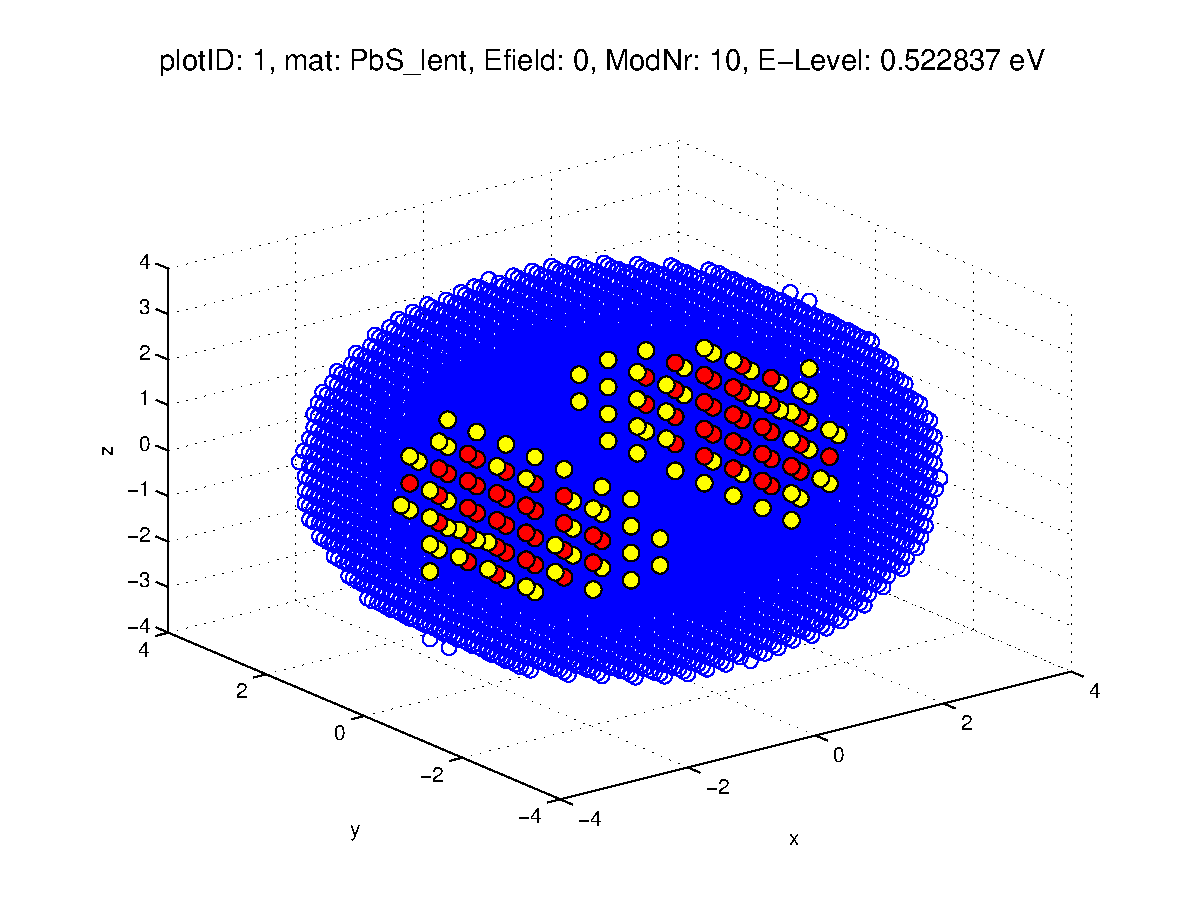
\includegraphics[width=150px]{Fig/Plots/r4CBmod10}
		\caption{}
	\end{subfigure}
	\begin{subfigure}{150px}
		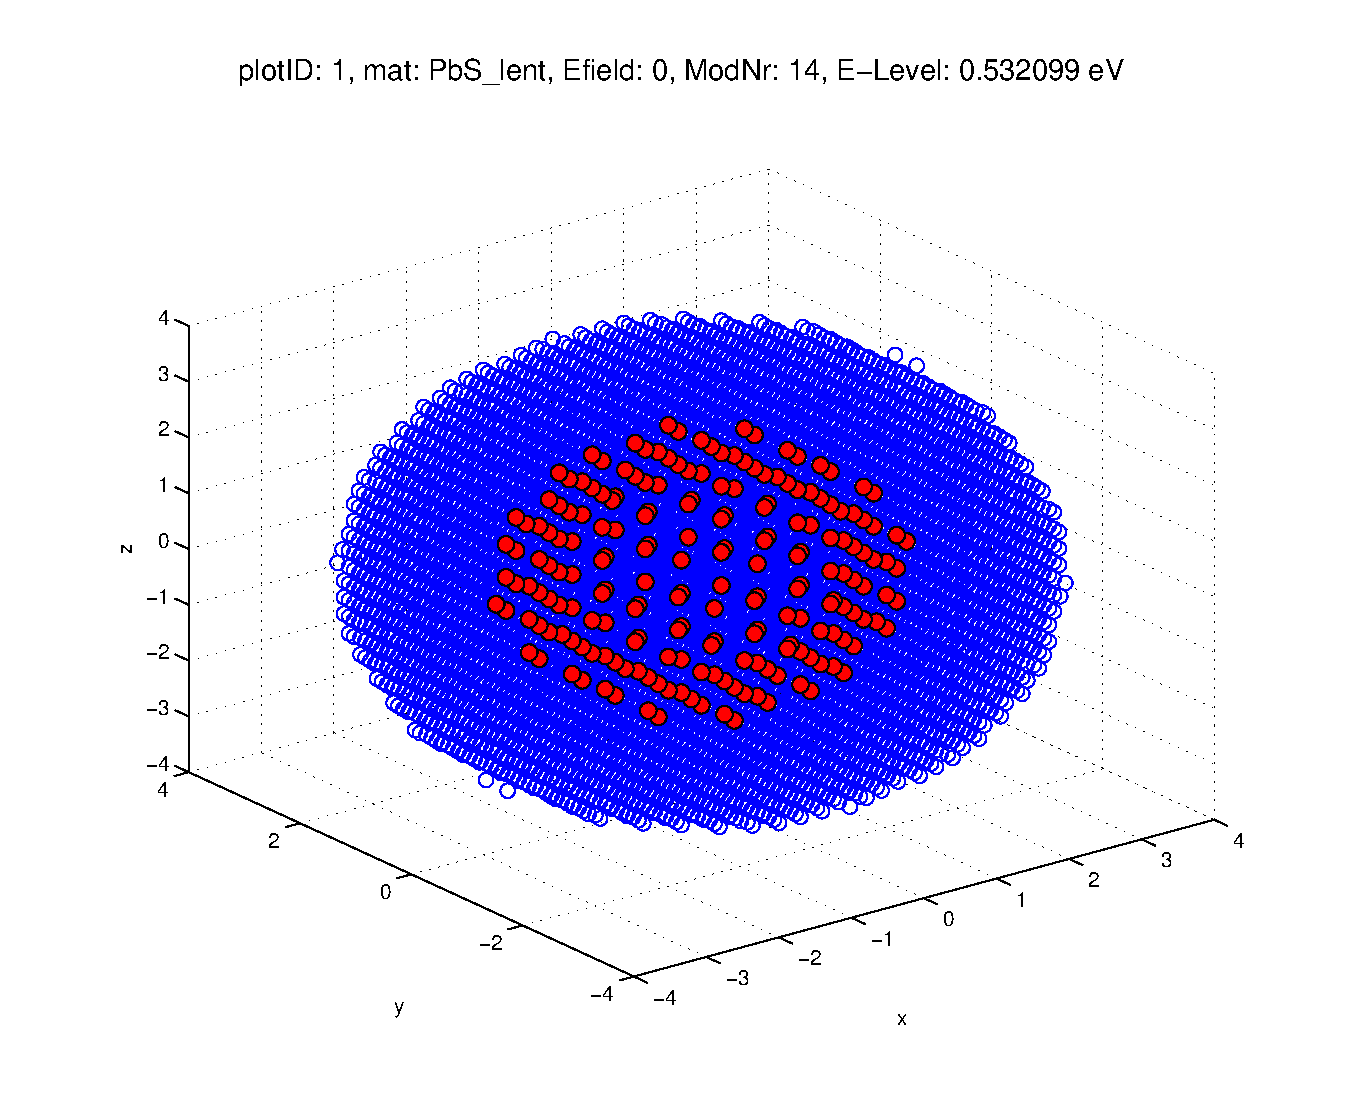
\includegraphics[width=150px]{Fig/Plots/r4CBmod14}
		\caption{}
	\end{subfigure}
	\begin{subfigure}{150px}
		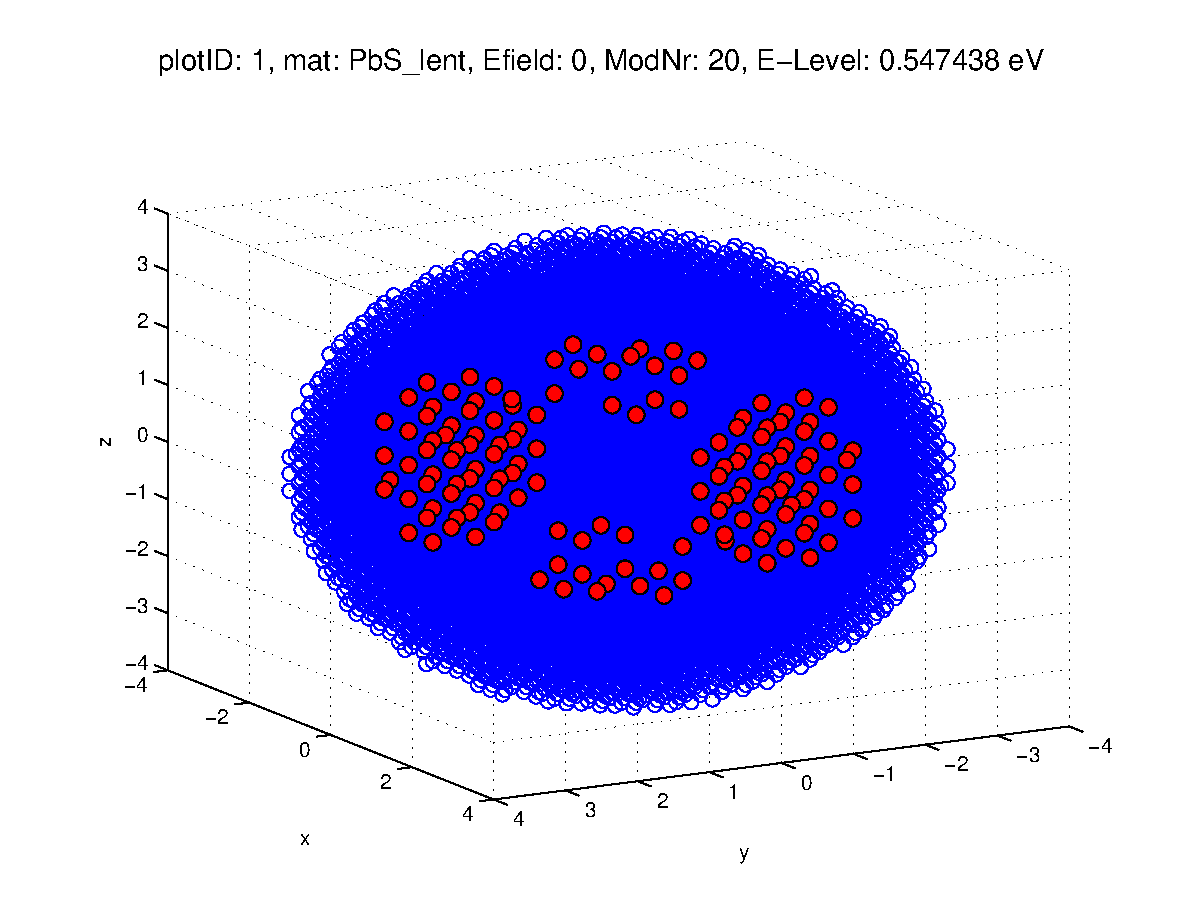
\includegraphics[width=150px]{Fig/Plots/r4CBmod20}
		\caption{}
	\end{subfigure}
	\caption{Probability density for higher energy states in an 8nm QD: barbell-shape (a), spherical shell-shape (b), crossed barbell-shape (c). In plots (b) and (c) the locations of medium high probability (yellow points) are not shown for clarity.}
	\label{fig:HigherModWaveFn}
\end{figure}
%

% TEXT
\begin{REMARK}
Although the term \textit{wave function} appears a lot in this section, the term is rather meant in the sense of \textit{probability density}, since the plots, on which the analysis is based, are more easily interpreted if they show probabilities instead of complex numbers.
\end{REMARK}

Sometimes, the wave functions of QDs are described in analogy to atomic orbitals, labeling them S, P, D and so on, with subscript e or h, denoting electron-like (conduction band) states or hole-like (valence band) states respectively. We will see how well this picture corresponds to the simulation.

The 8 energy states (`modes') closest to the band edge (for conduction and valence band respectively) have wave functions with spherical symmetry, where the highest probability density is in the center (fig.~\ref{fig:sphericalWaveFn}). This is in agreement with the 8 predicted $1S_{e,h}$ orbitals for PbS \cite[p.410]{ChemRev}.
	
The higher energy states show wave functions with more complex shapes. For example, a 8nm QD shows the following wave function shapes: After the 8 spherical conduction band states follow 4 (degenerate) states with barbell shape, in different orientations. Then 2 states with spherical shell shape. After that, 2 states with a shape similar to two crossed barbells. Then again 2 spherical shell-like states, followed by 2 ring-shaped wave functions, and so on (fig.~\ref{fig:HigherModWaveFn}). For the valence band states, the shapes are similar, although they do not occur in the same order (the same is true for QDs of different sizes).

\subsubsection{QDs smaller than 3nm}	

%FIGURES
\begin{figure}
	\centering
	\begin{subfigure}{200px}
		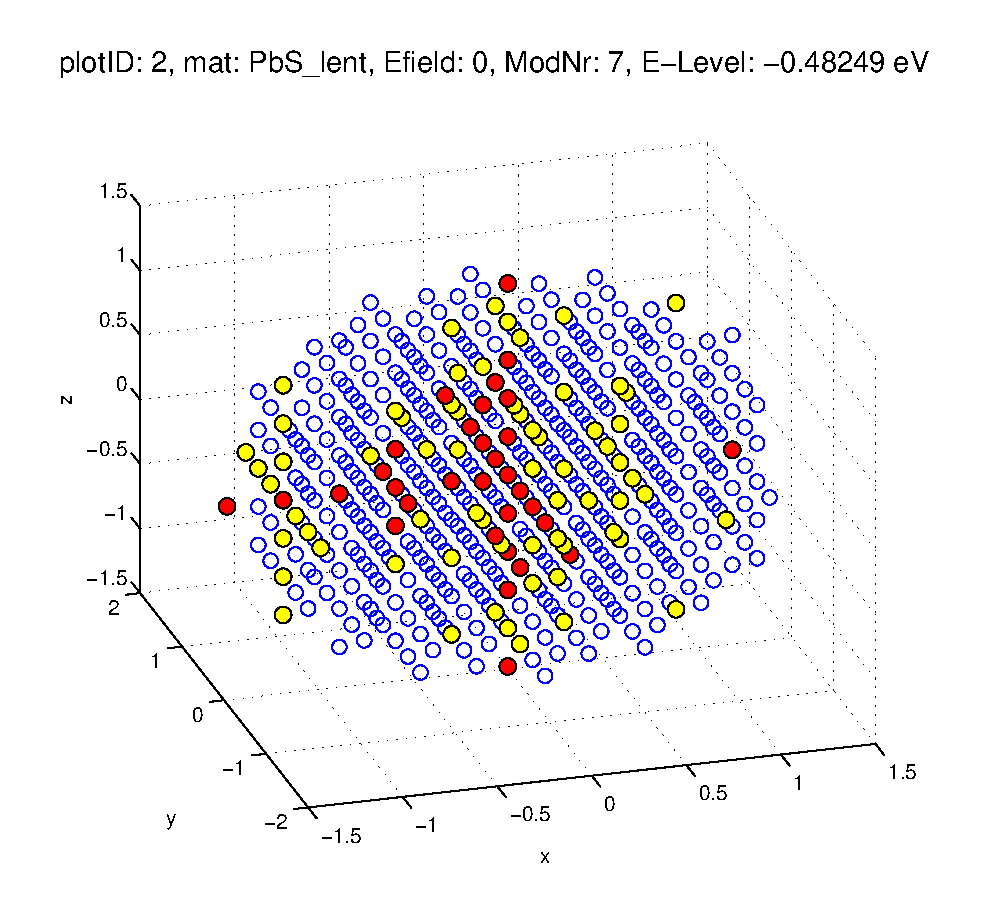
\includegraphics[width=200px]{Fig/Plots/r15VBmod7}
		\caption{3nm QD. 7th valence band state.}
	\end{subfigure}
	\begin{subfigure}{200px}
		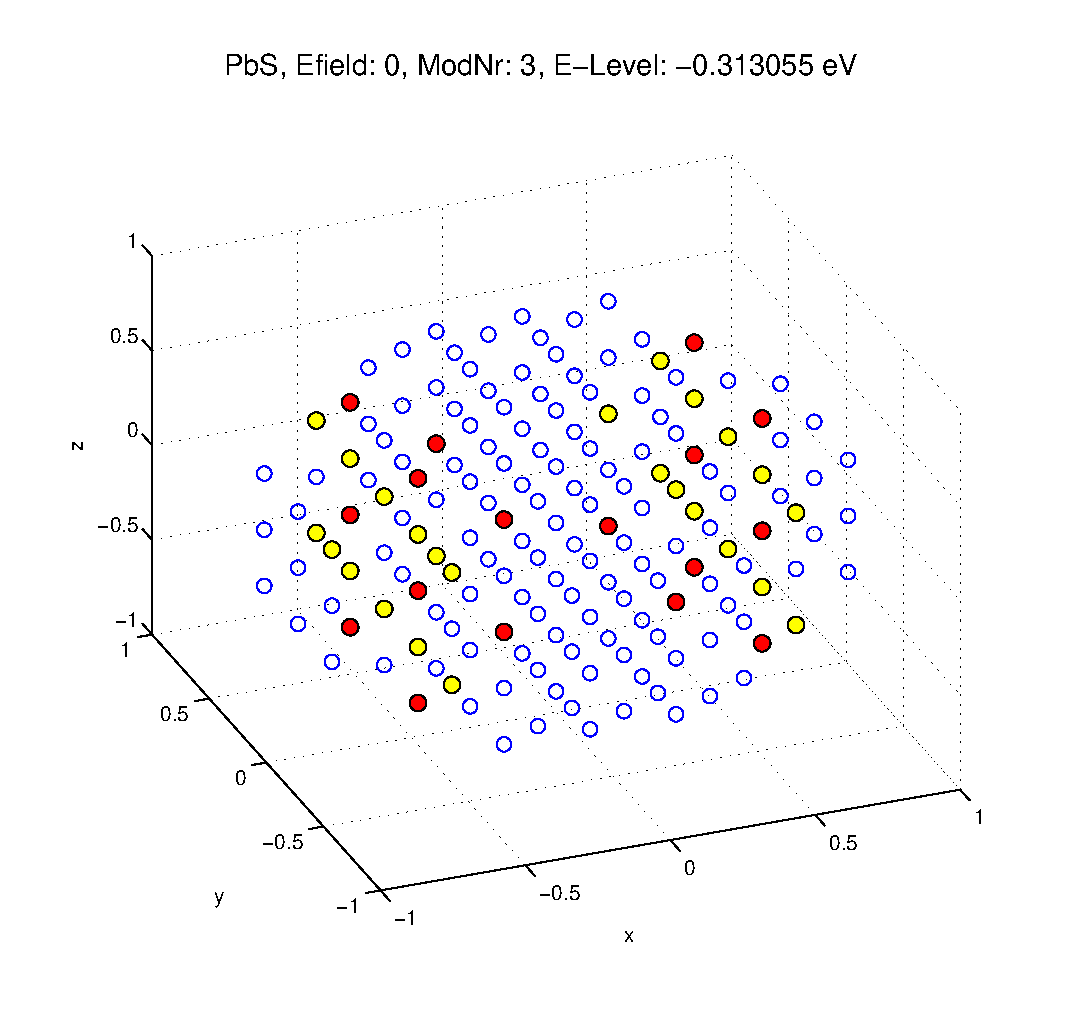
\includegraphics[width=200px]{Fig/Plots/r1VBmod3}
		\caption{2nm QD. 3rd valence band state.}
	\end{subfigure}
	\caption{Probability density for valence band states. The shape starts to deviate from the previously spherical shapes.}
	\label{fig:asymWaveFn}
\end{figure}


%TEXT
For QDs smaller than 3nm, the problem is that it is more difficult to see the shape of the wave function (too few atoms). Furthermore it is not clear how well this models a real QD, since the surface (and thus passivation of the surface) beginns to have an even bigger influence.
	
For a 2 and 3nm QDs, the 8 lowest conduction band states still remain more or less spherical. Whereas the valence band states start loose spherical symmetry. For a 3nm QD, mode 7 and 8 are already slightly asymetric (fig.~\ref{fig:asymWaveFn} (a)), and for the 2nm QD, even the modes 1 to 4 are clearly not spherical, but the wave function is rather localised at two sides (fig.~\ref{fig:asymWaveFn} (b)).
	
\FloatBarrier
\subsection{Influence of an electirc field}

%FIGURES
\begin{figure}
	\centering
	\begin{subfigure}{200px}
		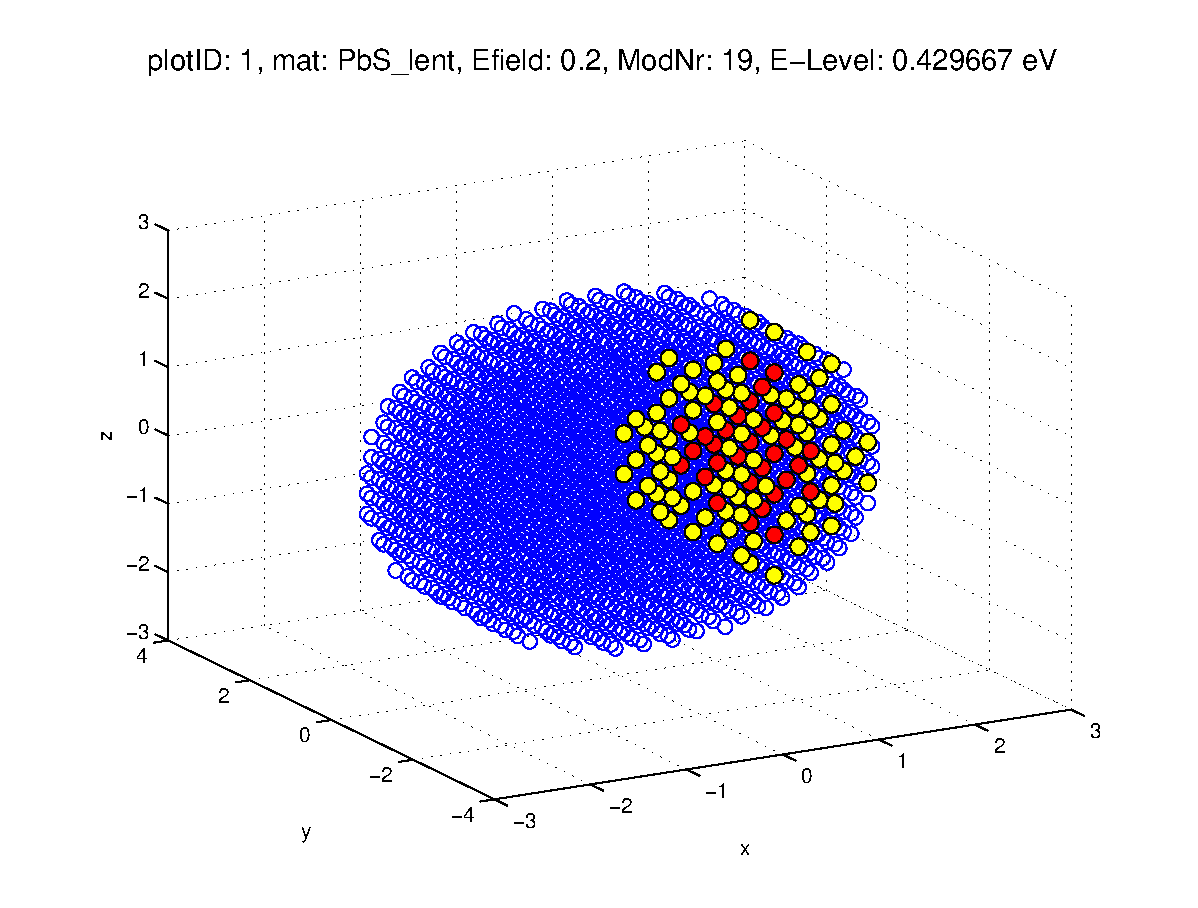
\includegraphics[width=200px]{Fig/Plots/r25v02CB}
		\caption{Conduction band state}
	\end{subfigure}
	\begin{subfigure}{200px}
		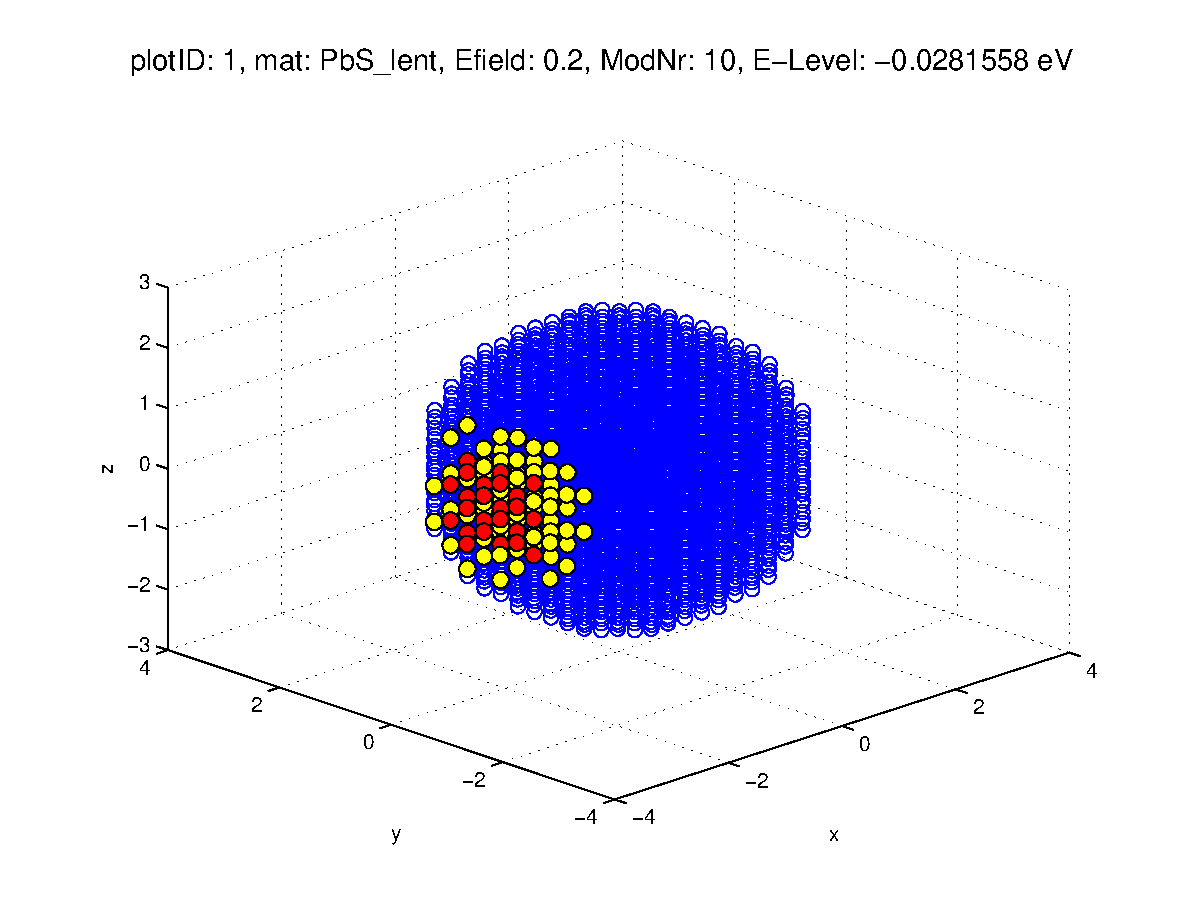
\includegraphics[width=200px]{Fig/Plots/r25v02VB}
		\caption{Valence band state}
	\end{subfigure}	
	\caption{Probability densities for a 5nm QD in an electic field of 0.2V/nm.}
	\label{fig:EfieldWaveFn}
\end{figure}
%
\begin{figure}
	\centering
	\begin{subfigure}{150px}
		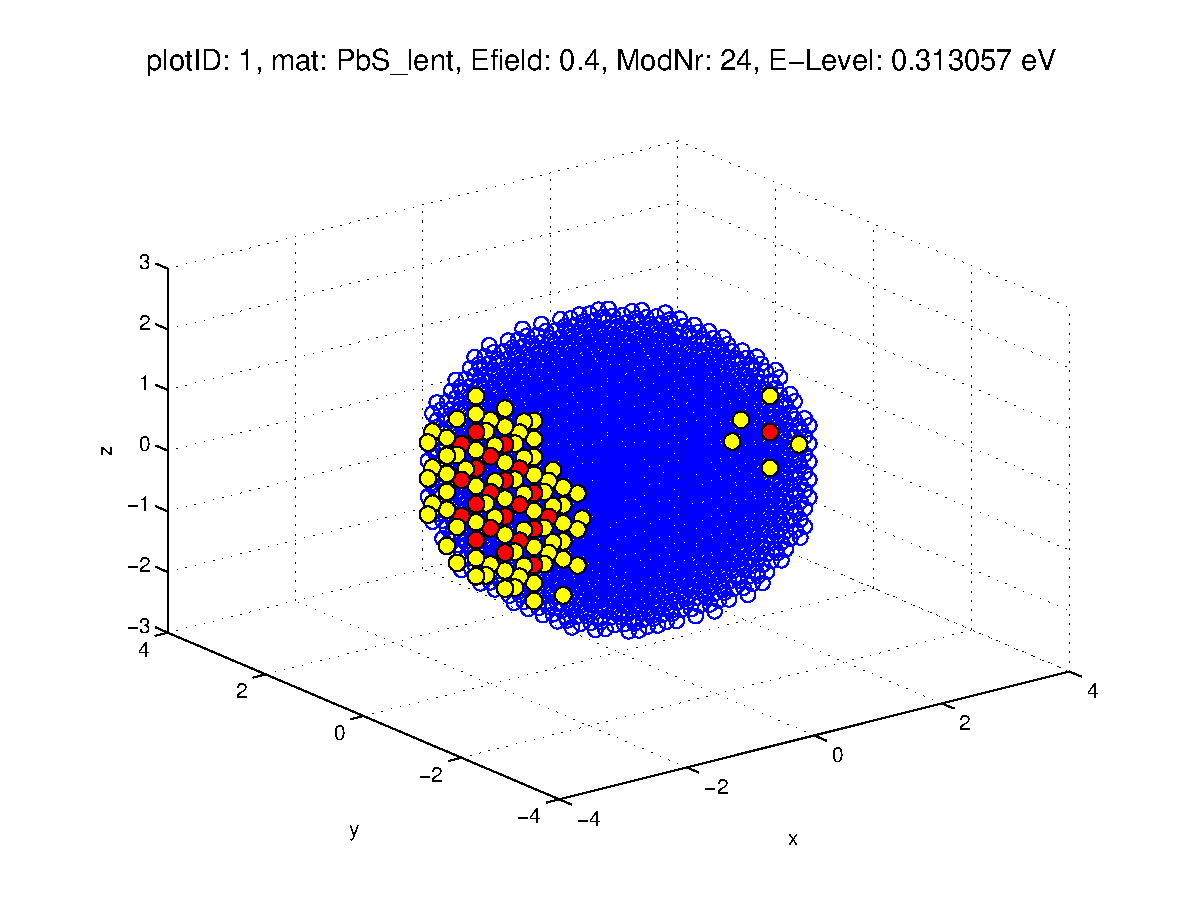
\includegraphics[width=150px]{Fig/Plots/r25v04Mod24}
		\caption{Eigenstate at 0.313057eV}
	\end{subfigure}
	\begin{subfigure}{150px}
		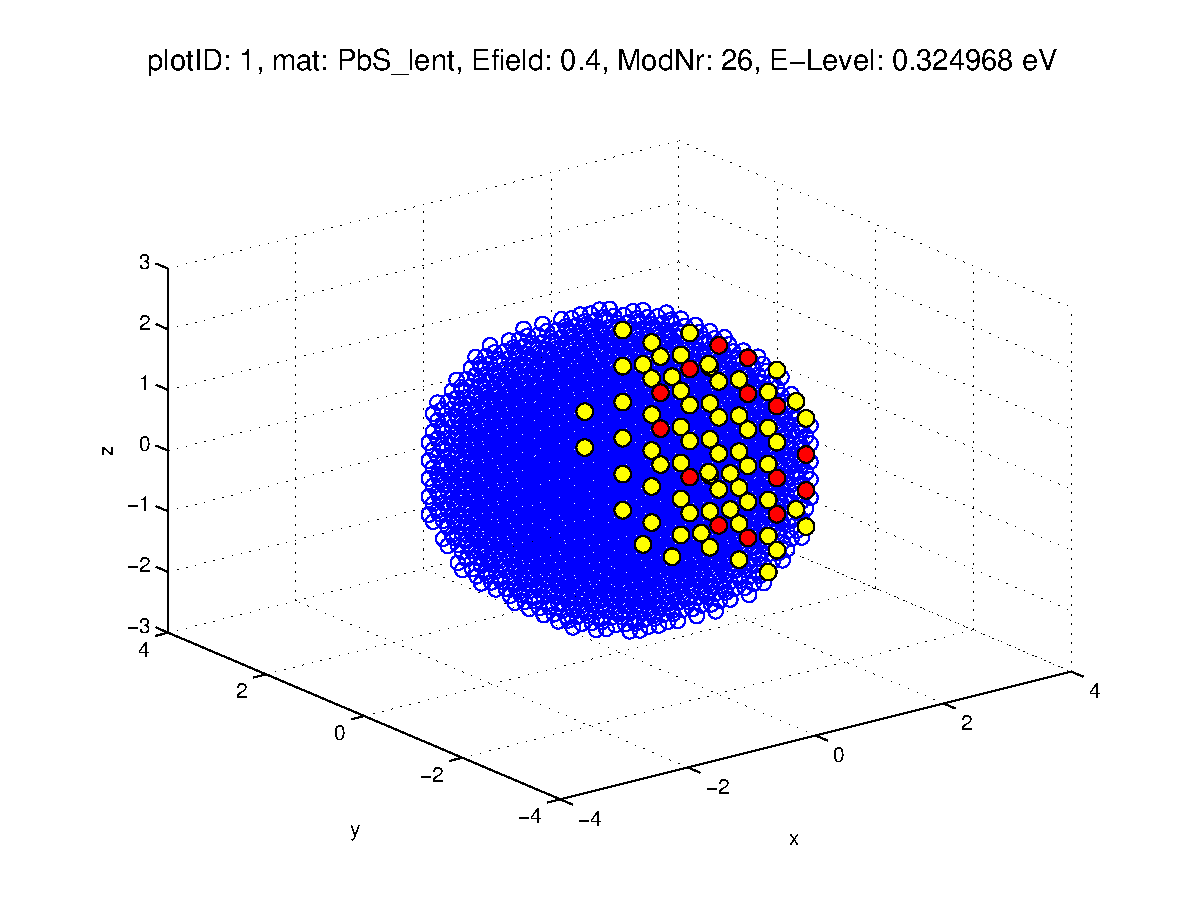
\includegraphics[width=150px]{Fig/Plots/r25v04Mod26}
		\caption{Eigenstate at 0.324968eV}
	\end{subfigure}
	\begin{subfigure}{150px}
		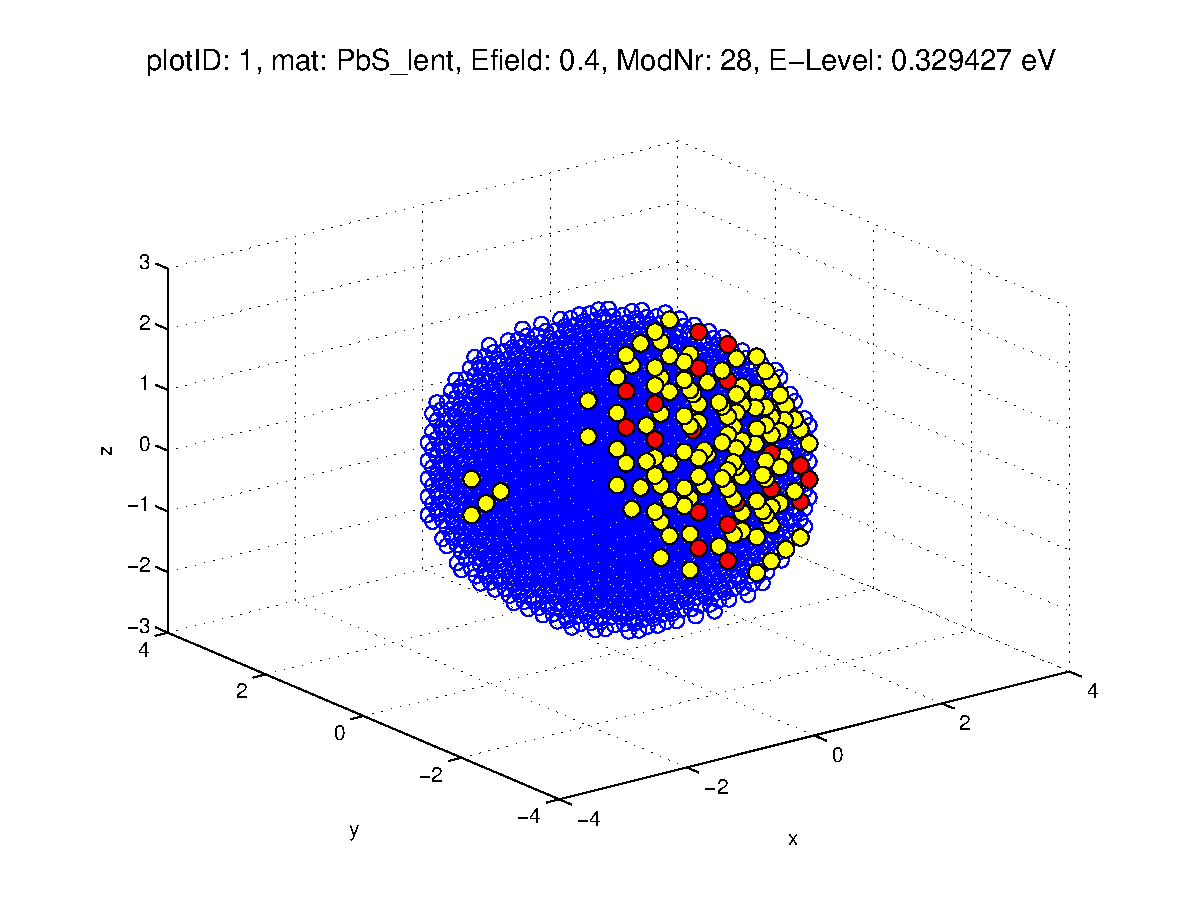
\includegraphics[width=150px]{Fig/Plots/r25v04Mod28}
		\caption{Eigenstate at  0.329427eV}
	\end{subfigure}
	\begin{subfigure}{150px}
		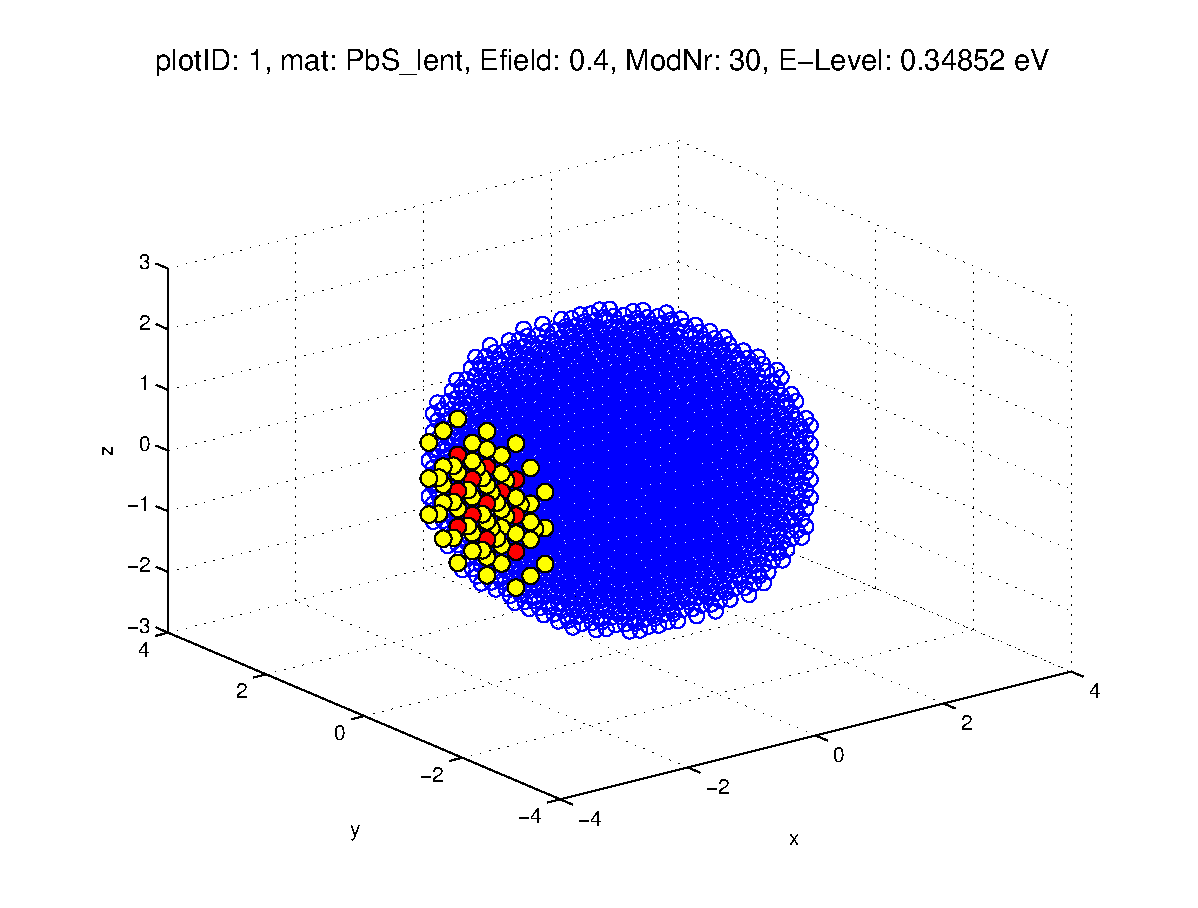
\includegraphics[width=150px]{Fig/Plots/r25v04Mod30}
		\caption{Eigenstate at 0.34852eV}
	\end{subfigure}
	\begin{subfigure}{150px}
		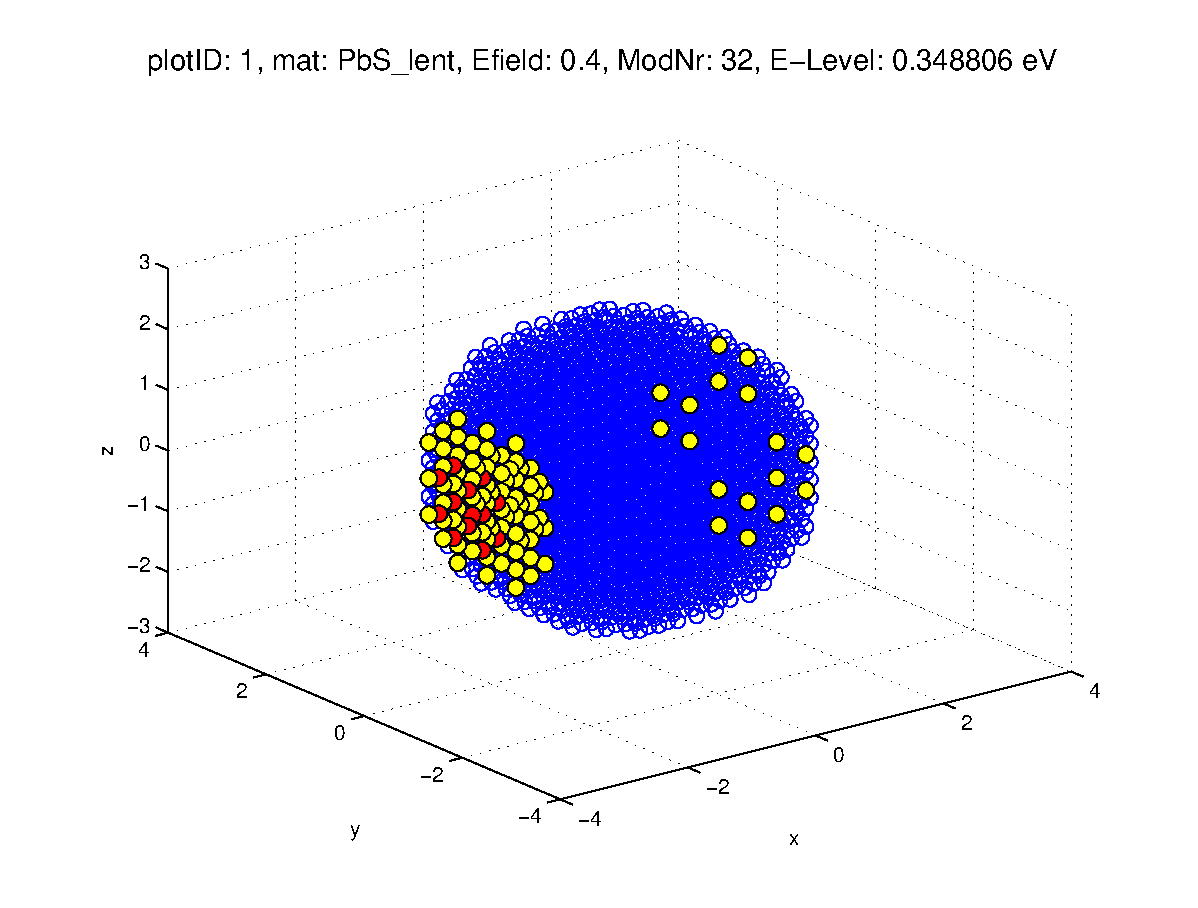
\includegraphics[width=150px]{Fig/Plots/r25v04Mod32}
		\caption{Eigenstate at 0.348806eV}
	\end{subfigure}
	\begin{subfigure}{150px}
		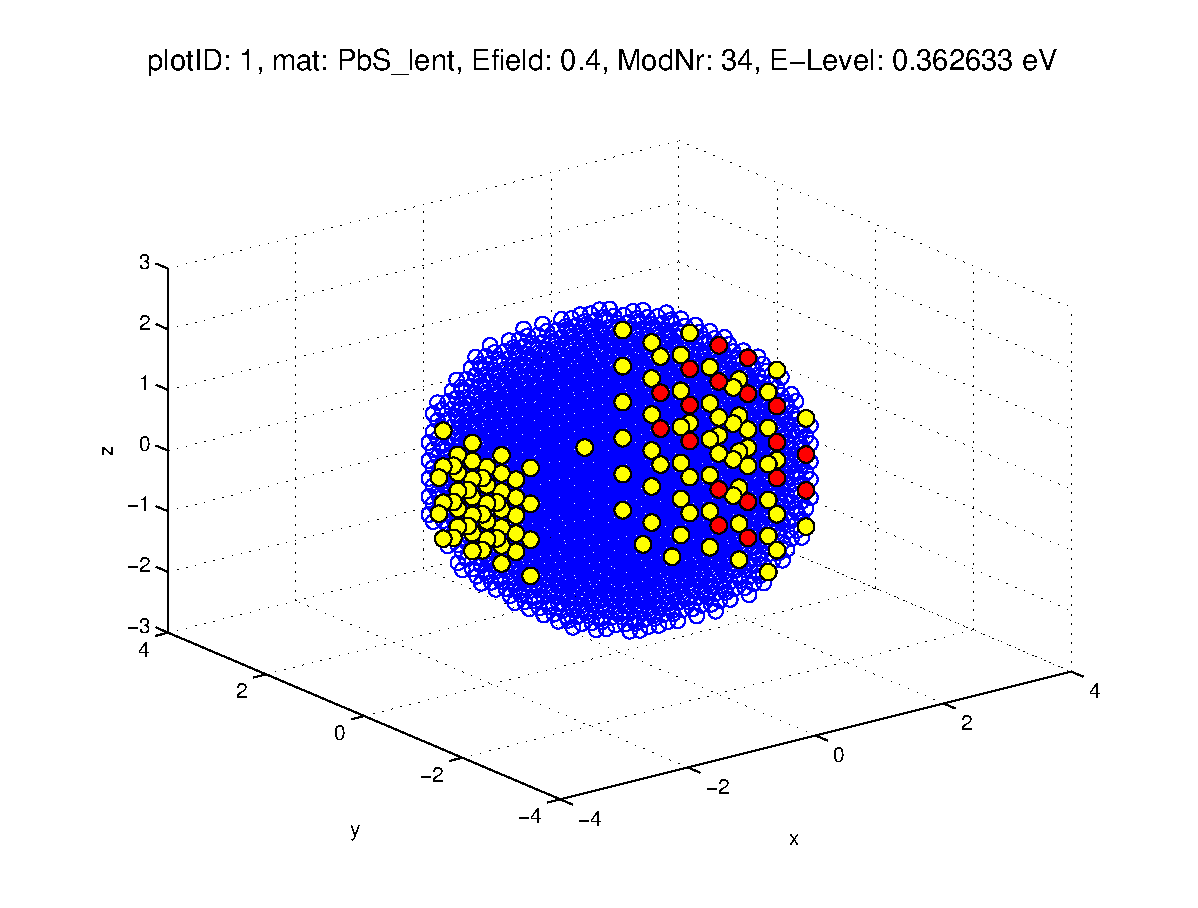
\includegraphics[width=150px]{Fig/Plots/r25v04Mod34}
		\caption{Eigenstate at 0.362633eV}
	\end{subfigure}
	\caption{Probability densities in the presence of a high electric field (0.4V/nm). Increasing energy from (a) to (f). Hole-like states (a),(d),(e) become mixed with electron-like states (b),(c),(f).}
	\label{fig:HighEfieldWaveFn}
\end{figure}


%TEXT
The presence of an electric field results in a shift of the wave function, i.e.~the maximum of the probability density is not in the center anymore and the spherical symetry of the 8 first states is broken (for conduction and valence band respectively). Furthermore, one can see that the valence band states really behave differently than conduction band states: The wave function is shifted in the opposite direction (fig.~\ref{fig:EfieldWaveFn}). This confirms that the valence band states are hole-like, similar to bulk semiconductor band theory. 
	
For larger electric fields the bandgap gets smaller, until it finally disappears, i.e. conduction and valence band states are not separated anymore. For example, for a 5nm  QD, the band gap disapperas for electirc fields larger than 0.35 V/nm (fig.~\ref{fig:EvsVolt}). The states close to the (former) band gap cannot be sepearted in conduction and valence band: as energy increases, some hole-like states are followed by electron-like (i.e.~conduction band-like) states, which in turn are followed by hole-like states and later again electron-like states (fig.~\ref{fig:HighEfieldWaveFn}).
	
Additionally, with higher electric fields, the wave functions seem not only to be shifted, but change shape: Some now look more like asymetric barbells or even stranger, ring-like shapes (fig.~\ref{fig:HighEfieldWaveFn} (a) and (f)).

\FloatBarrier

\section{Conclusions}

COMMENTS ABOUT BAND GAP

We have seen that larger PbS QDs have eightfold degenerate energy states at the band edges, whose wave functions have spherical symmetry, often named $S1_{e,h}$ orbitals. Higher energy states show more complex shaped wave functions. For QDs smaller than 3nm, the eightfold degeneracy is lost more and more, as well as the spherical symmetry of these wave functions. It is however questionable how close to reality the simulation of very small structures below 2nm are.
Under the influence of an electric field, the wave functions shift, according to their being hole- or electron-like in opposite directions.


